\documentclass{article}

\usepackage{natbib}
\usepackage{fullpage}

%\usepackage[nonatbib]{neurips_2020}

\usepackage[T1]{fontenc}    % use 8-bit T1 fonts
\usepackage{nicefrac}       % compact symbols for 1/2, etc.
\usepackage{microtype}      % microtypography
\usepackage{graphicx}

\usepackage{macro_math}
\usepackage{macro_fan}
\usepackage{stmaryrd}
\usepackage[us,12hr]{datetime}
\usepackage[utf8]{inputenc} % allow utf-8 input


\begin{document}

\title{Learning Multiple High-Dimensional Regression Tasks with Insights on Information Transfer}
\date{}
\maketitle
\date{{\ddmmyyyydate\today} at \currenttime}

\begin{abstract}
	Hard parameter sharing is a widely used approach to learn from multiple tasks in many applications, such as text classification. The idea is that all tasks share the same feature layer, while each task uses a specific output layer for prediction. Intuitively, the performance of hard parameter sharing depends on dataset properties such as their sample sizes. Yet, rigorously formulating such intuition can be technically challenging. This paper analyzes the generalization performance of hard parameter sharing in high-dimensional linear regression, where the sample size and feature dimension become increasingly large in a fixed ratio. We present tight generalization bounds for two canonical cases: (i) multiple tasks with the same feature covariates; (ii) two tasks with arbitrarily different sample sizes and covariance matrices. We also demonstrate that these estimates for the empirical loss of hard parameter sharing are incredibly accurate in modest dimensions. Finally, we explain several intriguing empirical phenomena. For example, increasing one task's sample size helps another task initially by reducing variance, but hurts eventually due to increasing bias. This suggests progressively adding data for optimizing hard parameter sharing, and we validate its efficiency in a text classification task.
%	Multi-task learning is a powerful approach in many applications such as image and text classification. Yet, there is little rigorous understanding of when multi-task learning outperforms single-task learning. In this work, we provide a rigorous study to answer the question in the high-dimensional linear regression setting. We show that a bias-variance tradeoff of multi-task learning determines the effect of information transfer, and develop new concentration bounds to analyze the tradeoff. Our key observation is that three properties of task data, namely \textit{task similarity}, \textit{sample ratio}, and \textit{covariate shift} can affect transfer in the high-dimensional linear regression setting. We relate each property to the bias and variance of multi-task learning and explain three negative effects with decreased task similarity,	increased sample ratio, and covariate shift under increased sample ratio. We validate the three effects on text classification tasks. Inspired by our theory, we show two practical connections of interest.
%	First, single-task results can help to understand when multi-task learning gives gains. Second, incrementally adding training data can mitigate negative transfer and improve multi-task training efficiency.
\end{abstract}

\section{Introduction}\label{sec introduction}

\iffalse
%Multi-task learning is an inductive learning mechanism to improve generalization performance using related task data.
%Many state-of-the-art results in computer vision and natural language processing are obtained using multi-task learning.
Multi-task learning is a powerful approach to improve performance for many tasks in computer vision, natural language processing, and other areas \cite{C97,ZY17,R17}.
%In multi-task learning, having related task data is fundamental to its performance.
%Multi-task learning is particularly powerful when there is limited labeled data for a task to be solved, meanwhile more labeled data from different but related tasks is available.
%By combining multiple information sources, it is possible to share all the information in the same model.
In many settings, multiple source tasks are available to help with predicting a particular target task.
\todo{clarify setting is different from traditional MTL}
%For example, many applications in , and many other areas have been achieved by learning from multiple tasks together.
The performance of multi-task learning depends on the relationship between the source and target tasks \cite{C97}.
%	We define that multi-task learning provides \textit{positive transfer} if it outperforms single-task learning, or \textit{negative transfer} otherwise.
When the sources are relatively different from the target, multi-task learning (MTL) has often been observed to perform worse than single-task learning (STL) \cite{AP16,BS17}, which is referred to as \textit{negative transfer} \cite{PY09}.
While many empirical approaches have been proposed to mitigate negative transfer \cite{ZY17}, a precise understanding of when negative transfer occurs remains elusive in the literature \cite{R17}.
%This phenomenon, known as \textit{negative transfer}, is fundamental to the understanding of multi-task learning.

%Inspired by the theory, we propose an incremental training schedule to improve multi-task training.
%We consider a setting where the target task has limited labeled data and show
%On the other hand, unless the structures across task data are well-understood, applying multi-task learning on several different datasets often result in suboptimal models (or negative transfer in more technical terms).

Understanding negative transfer requires developing generalization bounds that scale tightly with properties of each task data, such as its sample size.
This presents a technical challenge in the multi-task setting because of the difference among task features, even for two tasks.
For Rademacher complexity or VC-based techniques, the generalization error scales down as the sample sizes of all tasks increase, when applied to the multi-task setting \cite{B00,AZ05,M06,MPR16,WZR20}.
Without a tight lower bound for multi-task learning, comparing its performance to single-task learning results in vacuous bounds.
\todo{add more technical motivation (or maybe later)}
From a practical standpoint, developing a better understanding of multi-task learning in terms of properties of task data can provide guidance for downstream applications \cite{RH19}.
%For example, the sample sizes of all tasks are often assumed to be equal \cite{B00,LPTV09,LPVT11}.
%On the other hand, uneven sample sizes (or dominating tasks) have been empirically observed to cause negative transfer \cite{YKGLHF20}.
%The benefit of learning multi-task representations has also been studied for certain half-spaces \cite{} and sparse regression \cite{}.
%When all tasks are sufficiently similar, adding more labeled data improves the generalization performance for predicting a particular task \cite{WZR20}.

%\textbf{Setup and Main Results.}
In this work, we study the bias and variance of multi-task learning in the high-dimensional linear regression setting \cite{HMRT19,BLLT20}.
Our key observation is that three properties of task data, including \textit{task similarity}, \textit{sample ratio}, and \textit{covariate shift}, can affect whether multi-task learning outperforms single-task learning (which we refer to as \textit{positive transfer}).
As an example, we vary each property in Figure \ref{fig_model_shift_phasetrans} for two linear regression tasks and measure the improvement of multi-task learning over single-task learning for a particular task.
We observe that the effect of transfer can be either positive or negative as we vary each property.
These phenomena cannot be explained using previous techniques \cite{WZR20}.
The high-dimensional linear regression setting allows us to measure the three properties precisely.
Here we define each property for the case of two tasks, while our definition applies to general settings.
We refer to the first task as the source task and the second as the target task.
\squishlist
	\item \textbf{Task similarity:} Assume that both tasks follow a linear model with parameters $\beta_1, \beta_2\in\real^p$, respectively.
	We measure the distance between them by $\norm{\beta_1 - \beta_2}$.
	\item \textbf{Sample ratio:} Let $n_1 = \rho_1 \cdot p, n_2 = \rho_2 \cdot p$ be the sample size of each task, where $\rho_1, \rho_2>1$ are both fixed values that do not grow with $p$.
	We measure the source/target sample ratio by $\rho_1 / \rho_2$.
%	Importantly, $\rho_2$ can be a small constant (say $2$) to capture the need for more labeled data.
	\item \textbf{Covariate shift:} Assume that the task features are random vectors with positive semidefinite covariance matrices $\Sigma_1\in\real^{p\times p}$ and $\Sigma_2\in\real^{p\times p}$, respectively.
	%$x = \Sigma_i^{1/2}z$, where $z\in\real^p$ consists of i.i.d. entries with mean zero and unit variance, and is a positive semidefinite matrix.
	We measure covariate shift with matrix $\Sigma_1^{1/2}\Sigma_2^{-1/2}$.
\squishend

%The observations highlight the need to develop generalization bounds that scale tightly with properties of multiple tasks data.
% that only contains limited amount of labeled data.
%Following Hastie et al.  and Bartlett et al. \cite{},

%Let $n_i = \rho_i \cdot p$ denote the data size and $X_i\in\real^{n_i\times p}$ denote the features of task $i$.
%The labels of task $i$ are given by $Y_i = X_i\beta_i + \varepsilon_i$, where $\beta_i\in\real^p$ denotes task $i$'s ground truth parameters and $\varepsilon_i$ denotes i.i.d. random noise with mean zero and variance $\sigma^2$.
We consider a multi-task estimator obtained using a shared linear layer for all tasks and a separate output layer for each task \cite{WZR20}.
This two-layer model is inspired by a commonly used idea of hard parameter sharing in multi-task learning \cite{R17,MTDNN19}.
We consider the bias and variance of the multi-task estimator for predicting a target task and compare its performance to single-task learning.
%This corresponds to minimizing $ \sum_{i=1}^t \norm{X_i B W_i - Y_i}^2$.
%Let $\hat{\beta}_t^{\MTL}$ denote the optimal multi-task estimator for the target task, which is defined precisely in Section \ref{sec_prelim}.
%We revisit the bias-variance tradeoff of $\hat{\beta}_t^{\MTL}$.


\HZ{go to intro}
For a multivariate Gaussian random matrix, this result follows from the classical result for the mean of inverse Wishart distribution \cite{anderson1958introduction}.
For a non-Gaussian random matrix, this result can be obtained using the well-known Stieltjes transform method (cf. Lemma 3.11 of \citet{bai2009spectral}).
\fi


\section{Preliminaries}\label{sec_setup}

We describe the bias-variance tradeoff of our setting more formally.
Recall that we have $t$ labeled tasks available, denoted by $(X_1, Y_1), (X_2, Y_2), \dots, (X_t, Y_t)$, where $X_i\in\real^{n_i\times p}$ and $Y_i\in\real^{n_i}$ for $1\le i\le t$.
%Following \cite{HMRT19,BLLT20}, we assume that for each task $i = 1,2,\dots,t$,  every feature vector is generated as $x = \Sigma_i^{1/2} z$, where $z\in\real^p$ is a random vector with i.i.d. entries of mean zero and unit variance and $\Sigma_i\in\real^{p\times p}$ is a positive semidefinite matrix.
Without loss of generality, let the $t$-th task denote the target task.
For an estimator $\hat{\beta}\in\real^p$, we define the out-of-sample (prediction) loss as
	\begin{align*}
		\te_t(\hat{\beta}) \define \exarg{z}{\exarg{\varepsilon_t}{({(\Sigma_t^{1/2} z)}^{\top}\hat{\beta} - {(\Sigma_t^{1/2})}^{\top}\beta_t)^2}}
		= \exarg{\varepsilon_t}{(\hat{\beta} - \beta_t)^{\top}\Sigma_t(\hat{\beta} - \beta_t)}.
	\end{align*}
The single-task estimator $\hat{\beta}_t^{\STL}$ is given by $(X_t^{\top}X_t)^{-1}X_t^{\top}Y_t$.
The bias-variance trade-off \cite{HTF09} says
	\[ \te_t(\hat{\beta}) =
		\bignorm{\exarg{\varepsilon_t}{\hat{\beta}} - \beta_t}^2 + \exarg{\varepsilon_t}{\bignorm{\hat{\beta} - \exarg{\varepsilon_t}{\hat{\beta}}}^2}. \]
In order to study the trade-off between model-shift bias and variance reduction, we need tight concentration bounds to quantify both effects.
For this purpose, we consider the high-dimensional regime where $n_i$ is a fixed constant $\rho_i > 1$ times $p$ for every $1\le i\le t$, and $p$ is large.
%Recall that $n_i = \rho_i \cdot p$ and we assume $\rho_i > 1$ is a fixed constant for every $1\le i\le t$.

We focus on a setting where $\rho_t$ is a small constant.
This setting captures the need for adding more labeled data to reduce the test error of the target task.
A well-known result for this setting states that $\te_t(\hat{\beta}_t^{\STL}) = \sigma^2 \cdot \tr[(X_t^{\top}X_t)^{-1}\Sigma_t]$ is concentrated around $\frac {\sigma^2} {\rho_t - 1}$ (e.g. Chapter 6 of \cite{S07}), which scales with the data size and noise level of the target task.
However, this result only applies to the single-task setting.
Therefore, our goal is to extend this result to the multi-task setting.

To illustrate our intuition, we begin by considering the setting of two tasks with general covariance matrices.
Recall that $\hat{\beta}_t^{\MTL}$ is defined as $BW_t$ after solving equation \eqref{eq_mtl}.
We decompose the test error of $\hat{\beta}_{t}^{\MTL}$ on the target task into two parts (to be derived in Appendix \ref{app_proof_sec3}) as follows
\begin{align}
	\te_t(\hat{\beta}_t^{\MTL}) =& ~ \hat{v}^2 \bignorm{\Sigma_2^{1/2} (\hat{v}^2 X_1^{\top}X_1 + X_2^{\top}X_2)^{-1}X_1^{\top}X_1 (\beta_1 - \hat{v}\beta_2)}^2 \label{eq_te_model_shift} \\
	&+ \sigma^2\cdot \bigtr{(\hat{v}^2 X_1^{\top}X_1 + X_2^{\top}X_2)^{-1}\Sigma_2}, \label{eq_te_var}
\end{align}
where $\hat{v} = W_2 / W_1$ denotes the ratio of the output layer weights.
%Hence the bias of $\te_t(\hat{\beta}_t^{\STL})$ is zero and its test error is equal to variance, given by $$.

\textbf{Notations.}
When there is no ambiguity, we drop the subscript $t$ from $\te_t(\hat{\beta}_t^{\MTL})$ to $\te(\hat{\beta}_t^{\MTL})$ for simplicity.
We refer to the first task as the source task when there are only two tasks.
We call $M = \Sigma_1^{1/2}\Sigma_2^{-1/2}$ the covariate shift matrix.
%Same for $\hat{\beta}_t^{\STL}$.


\section{A Technical Tool to Quantify the Bias-Variance Trade-off}
\label{sec_main}

We develop a technical tool to derive $\te(\hat{\beta}_t^{\MTL})$ that only depends on the qualities of task data such as data sizes and covariance matrices, for two tasks with general covariances.
Then, we extend the result to more than two tasks that share the same features but have different labels.
Finally, we show a sharp bias-variance tradeoff for transfer learning settings.


\subsection{A Key Lemma using Random Matrix Theory}\label{label_rmt}


\begin{lemma}[Informal statement of Lemma \ref{lem_cov_shift}]\label{lem_cov_shift_informal}
	Suppose $X_1=Z_1\Sigma_1^{1/2}\in \R^{n_1\times p}$ and $X_2=Z_2\Sigma_2^{1/2}\in \R^{n_2\times p}$ with $\rho_1=n_1/p>1$ and $\rho_2=n_2/p>1$.
	Let $M = \Sigma_1^{1/2}\Sigma_2^{-1/2}$ and $\lambda_1, \lambda_2, \dots, \lambda_p$ be the singular values of $M^{\top}M$ in descending order.
	For any constant $\e>0$, w.h.p. over the randomness of $X_1, X_2$, we have that
	\begin{align*}
		\bigtr{(X_1^{\top}X_1 + X_2^{\top}X_2)^{-1}\Sigma_2} = \frac{1}{\rho_1+\rho_2}\cdot \frac1p\bigtr{ (a_1 \Sigma_1 + a_2\Sigma_2)^{-1} \Sigma_2} +\bigo{\|\Sigma_2\| p^{-1/2+\epsilon}},
	\end{align*}
where $(a_1, a_2)$ is the solution to the following deterministic equations:
	\begin{align*}
		a_1 + a_2 = 1- \frac{1}{\rho_1 + \rho_2},\quad a_1 + \frac1{\rho_1 + \rho_2}\cdot \frac{1}{p}\sum_{i=1}^p \frac{\lambda_i^2 a_1}{\lambda_i^2 a_1 + a_2} = \frac{\rho_1}{\rho_1 + \rho_2}.
	\end{align*}
\end{lemma}

\subsection{Applications to Multi-Task and Transfer Learning}

\textbf{Multi-task learning.} applies to the setting of two tasks where their covariance matrices may be arbitrarily different.
The above result also applies to the setting of more than two tasks with the same covariates.
%We extend the above result to any number of tasks that have the same covariates.
%In this section we consider the setting with $k$ many that have the same covariates.
Since the tasks all have the same number of datapoints and covariance matrix, the trade-off between model shift bias and variance will be captured by their task models $\set{\beta_i}_{i=1}^k$.
%For this setting, we derive solutions for the multi-task training and the transfer learning setting that match our insights qualitatively from Section \ref{sec_denoise}.
%Let $B^{\star} = [\beta_1, \beta_2, \dots, \beta_k] \in\real^{p\times k}$ denote the underlying task model parameters.
The formal statement is stated in Theorem \ref{thm_many_tasks} and its proof can be found in Appendix \ref{app_proof_many_tasks}.
%The technical crux of our approach is to derive the asymptotic limit of $\te(\hat{\beta}_t^{\MTL})$ in the high-dimensional setting, when $p$ approaches infinity.
We derive a precise limit of $\bigtr{(X_1^{\top}X_1 + X_2^{\top}X_2)^{-1}\Sigma_2}$, which is a deterministic function that only depends on $\Sigma_1, \Sigma_2$ and $n_1/p, n_2/p$ (see Lemma \ref{lem_cov_shift} in Appendix \ref{app_proof_main} for the result).
Based on the result, we show how to determine positive versus negative transfer as follows.

\begin{theorem}[Informal statement of Theorem \ref{thm_model_shift}]\label{thm_main_informal}
	Let $X_i \in\real^{n_i \times p}$ and $Y_i = X_i\beta_i + \varepsilon_i$, for $i = 1, 2$.
	Suppose that $n_1 = \rho_1 p$ and $n_2 = \rho_2 p$, where $\rho_1>1$ and $\rho_2 >1$ are fixed constants.
	There exists two deterministic functions $\Delta_{\beta}$ and $\Delta_{\vari}$ and a small deterministic error $\delta$ that only depend on $\set{\hat{v}, \Sigma_1^{}, n_1, n_2, \beta_1, \beta_2}$ such that
	\begin{itemize}
		\item If $\Delta_{\vari} - \Delta_{\beta} \ge \delta$, then whp $\te(\hat{\beta}_t^{\MTL}) < \te(\hat{\beta}_t^{\STL})$.
		\item If $\Delta_{\vari} - \Delta_{\beta} \le \delta$, then whp $\te(\hat{\beta}_t^{\MTL}) > \te(\hat{\beta}_t^{\STL})$.
	\end{itemize}
\end{theorem}

Theorem \ref{thm_main_informal} shows nearly tight bounds on the trade-off between model-shift bias and variance reduction.
%determined by the covariate shift matrix and the model shift.
The bounds get tighter and tighter as $\rho_1$ increases.
While the general form of $\Delta_{\vari}$ and $\Delta_{\beta}$ can be quite complex, we will show that they provide nice interpretation for simplified settings later on in Section \ref{sec_insight}.
A formal version of Theorem \ref{thm_main_informal} is presented in Theorem \ref{thm_model_shift} and its proof is presented in Appendix \ref{app_proof_main}.

\textbf{Transfer learning.}
We extend the intuition behind Theorem \ref{thm_main_informal} to transfer learning settings.
We provide an analysis of the transfer function of Taskonomy \cite{ZSSGM18} using our setup.
Specifically, the source task encoder consists of the representations learnt from one or more source tasks.
The transfer function then tries to fit the target task data to the source task encoder.
For more details, we refer the reader to Figure 4 in Taskonomy.

We map the procedure to our setup as follows.
First, we obtain the single-task estimator $\hat{\beta}_i$ from the source tasks, for $1\le i \le t-1$.
This forms the shared representation $B = [\hat{\beta}_1,\hat{\beta}_2,\dots,\hat{\beta}_{t-1}]$.
Then, we learn the output layer $W_t$ on the target task by minimizing the following objective
\begin{align}
	g(W_t) = \bignorm{X_t B W_t - Y_t}^2.
\end{align}
After solving $W_t$, we use $\hat{\beta}_t^{\TL} = B W_t$ as the estimator for the target task.
By comparing $\te(\hat{\beta}_t^{\TL})$ to $\te(\hat{\beta}_t^{\STL})$, we observe a similar trade-off between model-shift bias and variance reduction for this setting.
%We use our tools to compare $\te(B W_t)$ to $\te(\beta_t^{\STL})$.
The formal statement is presented in Theorem \ref{prop_taskonomy} and its proof in Appendix \ref{app_proof_sec4}.



\section{The De-Noising Effect of Multi-Task Learning}


In this part, we shall establish the intuition that adding more data helps in multi-task learning by reducing the variance of the estimator.
We achieve this through tight generalization bounds obtained from random matrix theory.
We focus the case of two tasks to provide a complete picture on how covariate and model shifts can affect the type of transfer.

Recall that the test error of $\hat{\beta}_{t}^{\MTL}$ consists of two parts
\begin{align}
	\te(\hat{\beta}_t^{\MTL}) = \hat{w}^2 \bignorm{\Sigma_2^{1/2} (\hat{w}^2 X_1^{\top}X_1 + X_2^{\top}X_2)^{-1}X_1^{\top}X_1 (\beta_s - \hat{w}\beta_t)}^2 + \sigma^2\cdot \bigtr{(\hat{w}^2 X_1^{\top}X_1 + X_2^{\top}X_2)^{-1}\Sigma_2}. \label{eq_te_model_shift}
\end{align}
It is not hard to show that the variance of $\hat{\beta}_t^{\MTL}$ is reduced compared to $\hat{\beta}_t^{\STL}$ (following the argument of Proposition \ref{prop_monotone}), i.e.
\[ \sigma^2\cdot \bigtr{(\hat{w}^2 X_1^{\top}X_1 + X_2^{\top}X_2)^{-1}\Sigma_2} \le \sigma^2\cdot \bigtr{(X_2^{\top}X_2)^{-1}\Sigma_2}. \]
Because of model shift however, i.e. $\beta_s \neq \beta_t$.
We can no longer guarantee that $\te(\hat{\beta}_{t}^{\MTL}) \le \te(\hat{\beta}_t^{\STL})$.
The main result of this part show deterministic conditions under which we get positive or negative transfer.
And the conditions depend only on the covariate shift matrix $M$, the difference of the task models, and the number of per-task data points.
In order to characterize $\te(\hat{\beta}_t^{\MTL})$ and $\te(\hat{\beta}_t^{\STL})$, the technical crux of our approach relies on deriving the limit of the trace of matrix inverse in the high-dimensional setting.
To illustrate the idea, we observe that by using Lemma \ref{lem_minv}, we have that
\[ \te(\hat{\beta}_t^{\STL}) = \frac{\sigma^2}{n_2 - p}\bigtr{\Sigma_2^{-1}}. \]
We shall also derive the limit of $\te(\hat{\beta}_t^{\MTL})$.
\todo{write a brief technical overview}

%In this case, $\beta_s$ and $\beta_t$ are different.
%, or implicitly add a regularization on $B$.
%\todo{We focus on the former case in this section.}
%, we consider the case when $r=1$ since there are only two tasks.
%We begin by considering the simplified equation \eqref{eq_mtl_basic} to solve for the target task.
%This is equivalent to setting $W_i = 1$ for the two tasks in equation \eqref{eq_mtl}.
%The result of this simplified setting will set up the ground for solving equation \eqref{eq_mtl} when we also optimize $W_1$ and $W_2$.
%By putting the two tasks together, we get
%\begin{align*}
%	\hat{\beta}_{s,t} &= (X_1^{\top}X_1 + X_2^{\top}X_2)^{-1} (X_1^{\top}Y_1 + X_2^{\top}Y_2) \\
%	&= (X_1^{\top}X_1 + X_2^{\top}X_2)^{-1} \bigbrace{(X_1^{\top}X_1\beta_s + X_2^{\top}X_2\beta_t) + (X_1^{\top}\varepsilon_1 + X_2^{\top}\varepsilon_2)} \\
%	&= \beta_t + (X_1^{\top}X_1 + X_2^{\top}X_2)^{-1}\bigbrace{X_1^{\top}X_1(\beta_s - \beta_t) + (X_1^{\top}\varepsilon_1 + X_2^{\top}\varepsilon_2)}
%\end{align*}
%Hence
%\begin{align}
%	\err(\hat{\beta}_{s,t})
%	&= \bignorm{(X_1^{\top}X_1 + X_2^{\top}X_2)^{-1} X_1^{\top}X_1 (\beta_s - \beta_t)}^2
%	+ \sigma^2 \bigtr{(X_1^{\top}X_1 + X_2^{\top}X_2)^{-1}}, \text{ and} \\
%	\te(\hat{\beta}_{s,t})
%	&= \bignorm{\Sigma_2^{1/2} (X_1^{\top}X_1 + X_2^{\top}X_2)^{-1} X_1^{\top}X_1 (\beta_s - \beta_t)}^2 + \sigma^2\cdot \bigtr{(X_1^{\top}X_1 + X_2^{\top}X_2)^{-1}\Sigma_2} \label{eq_te_model_shift}
%\end{align}



\todo{For technical reasons, we will consider the test error.}


We state our main result for two tasks with both covariate and model shift in the following theorem.

\begin{theorem}\label{thm_model_shift}
	Let $n_1, n_2$ be the number of data points for the source, target task, respectively.
	Let $\hat{w}$ denote the optimal solution for the ratio $w_1/w_2$ in equation \eqref{eq_val_mtl}.
	Let ${M} = \hat{w} \Sigma_1^{1/2}\Sigma_2^{-1/2}$ denote the weighted covariate shift matrix.
	Denote by ${\lambda}_1, {\lambda}_2, \dots, {\lambda}_p$ the singular values of ${M}^{\top}{M}$.
	The information transfer is solely determined by two deterministic quantities $\Delta_{\beta}$ and $\Delta_{\vari}$, which show the change of model shift bias and variace, respectively.
	With high probability we have
	\begin{align}
	 	\te(\hat{\beta}_{t}^{\MTL}) \le \te(\hat{\beta}_t^{\STL}) \text{ when: } &\Delta_{\vari} - \Delta_{\beta} \ge \left(\bigbrace{1 + \sqrt{\frac{p} {n_1}}}^4 - 1 \right) \delta \label{upper}\\
		\te(\hat{\beta}_t^{\MTL}) \ge \te(\hat{\beta}_t^{\STL}) \text{ when: } &\Delta_{\vari} - \Delta_{\beta} \le -2\bigbrace{2\sqrt{\frac {p}{n_1}} + \frac{p}{n_1}} \delta, \label{lower}
	\end{align}
	where $\delta = \norm{Z} \cdot \norm{\Sigma_1^{1/2}(\beta_s - \hat{w}\beta_t)}^2$ with $Z = \frac{n_1^2}{(n_1 + n_2)^2}\cdot{M} \frac{(1 + a_3)\id + a_4 {M}^{\top}{M}}{(a_2 + a_1 {M}^{\top}{M})^2} {M}^{\top}$, and
	\begin{align*} %\bigtr{{\Sigma_2^{-1}}}
		\Delta_{\vari} &\define {\sigma^2}\bigbrace{\frac{p}{n_2 - p} -  \frac{1}{n_1 + n_2} \bigtr{(a_1 M^{\top}M + a_2\id)^{-1}} } \\
		\Delta_{\beta} &\define (\beta_s - \hat{w}\beta_t)^{\top} \Sigma_1^{1/2} Z \Sigma_1^{1/2} (\beta_s - \hat{w}\beta_t),
	\end{align*}
%	{\color{blue}To write the bounds in the form \eqref{upper} and \eqref{lower}, we have to define $\wh w$ as the minimizer of
%	$$\frac{\sigma^2}{n_1 + n_2} \bigtr{\frac1{a_1(w) M(w)^{\top}M(w) + a_2(w)\id}}+ \Delta_\beta(w).$$
%	Otherwise, the two bounds has to be written into the form
%	\begin{align*}
%	{\sigma^2}\frac{p}{n_2 - p}\ge \min_w \left\{\frac{\sigma^2}{n_1 + n_2} \bigtr{\frac1{a_1(w) M(w)^{\top}M(w) + a_2(w)\id}} + \Delta_\beta(w)+ \left(\bigbrace{1 + \sqrt{\frac{p} {n_1}}}^4 - 1 \right) \delta(w)\right\},
%	\end{align*}
%	and
%	\begin{align*}
%	{\sigma^2}\frac{p}{n_2 - p}\le \min_w \left\{\frac{\sigma^2}{n_1 + n_2} \bigtr{\frac1{a_1(w) M(w)^{\top}M(w) + a_2(w)\id}}+ \Delta_\beta(w) - 2\bigbrace{2\sqrt{\frac {p}{n_1}} + \frac{p}{n_1}} \delta(w)\right\}.
%	\end{align*}
%	}
%
%
	and $a_1, a_2, a_3, a_4$ are the solutions of the following linear equations
	\begin{gather}
		 a_1 + a_2 = 1- \frac{p}{n_1 + n_2},~ a_1 + \sum_{i=1}^p \frac{a_1}{(n_1 + n_2)(a_1 + a_2/ \lambda_i^2)} = \frac{n_1}{n_1 + n_2}, \label{eq_a2} \\
		\left(\frac{n_2}{a_2^2}- \sum_{i=1}^p \frac{1}{ (a_2 + \lambda_i^2a_1)^2  }\right) a_3 -  \left(\sum_{i=1}^p \frac{  \lambda_i^2 }{ (  a_2 + \lambda_i^2a_1)^2  }\right)a_4
		= \sum_{i=1}^p \frac{1 }{ (  a_2 + \lambda_i^2a_1)^2  }, \label{eq_a3} \\
		\left(\frac{n_1}{a_1^2} -  \sum_{i=1}^p \frac{\lambda_i^4   }{  (a_2 + \lambda_i^2a_1)^2  }\right)a_4 -\left(\sum_{i=1}^p \frac{\lambda_i^2  }{  (a_2 + \lambda_i^2a_1)^2  }\right)a_3
		= \sum_{i=1}^p \frac{\lambda_i^2 }{  (a_2 + \lambda_i^2a_1)^2  }. \label{eq_a4}
	\end{gather}
\end{theorem}


%	We have the following conditions that guarantee the type of transfer we can get under model shift.
%	\begin{itemize}

%		\item {\bf Negative transfer:} we have $\te(\hat{\beta}_{s,t}) \ge \te(\hat{\beta}_t)$ when
%			\begin{align}
%				\Delta_{\vari} \le \bigbrace{1 - 4\sqrt{\frac{p}{n_1}} - \frac{2p}{n_1}} {\Delta_{\beta}}
%			\end{align}
%	\end{itemize}
%	\begin{align}
%		{\Delta_{\vari}} \ge \bigbrace{1 + \sqrt{\frac{p}{n_1}}}^2 {\Delta_{\beta}},
%\label{eq_model_shift_pos}
%	\end{align}
%	where
%{\cob
%We have that
%	\begin{align*}
%		&~ {\bignorm{\Sigma_2^{1/2} (X_1^{\top}X_1 + X_2^{\top}X_2)^{-1} X_1^{\top}X_1 (\beta_s - \beta_t)}} \\
%		&\le ~ \Delta_\beta^{1/2}+ \left\|M\frac{(1 + a_3)\id + a_4 M^{\top}M}{(a_1 + a_2 M^{\top}M)} M^{\top}\right\|_{op}^{1/2} \|\Sigma_1^{1/2} (\beta_s - \beta_t)\|_2 \left( 2\sqrt{\frac{p} {n_1}} + \frac{p}{n_1}\right),\\
%		\end{align*}
%		and
%	\begin{align*}
%		&~ {\bignorm{\Sigma_2^{1/2} (X_1^{\top}X_1 + X_2^{\top}X_2)^{-1} X_1^{\top}X_1 (\beta_s - \beta_t)}} \\
%		&\ge ~ \Delta_\beta^{1/2}- \left\|M\frac{(1 + a_3)\id + a_4 M^{\top}M}{(a_1 + a_2 M^{\top}M)} M^{\top}\right\|_{op}^{1/2} \|\Sigma_1^{1/2} (\beta_s - \beta_t)\|_2 \left( 2\sqrt{\frac{p} {n_1}} + \frac{p}{n_1}\right),
%	\end{align*}
%	In the case where the entries of $\beta_s-\beta_t$ are i.i.d. random variables and $\Sigma_1=\id$, we have
%\begin{align*}
%		& \Delta_\beta\left( 1-\sqrt{\frac{p}{n_1}}\right)^4 \le ~ {\bignorm{\Sigma_2^{1/2} (X_1^{\top}X_1 + X_2^{\top}X_2)^{-1} X_1^{\top}X_1 (\beta_s - \beta_t)}}^2 \le ~
%\Delta_\beta\left( 1+\sqrt{\frac{p}{n_1}}\right)^4.
%		\end{align*}
%	}

Theorem \ref{thm_model_shift} shows upper and lower bounds that guarantee positive transfer, which is determined by the change of variance $\Delta_{\vari}$ and a certain model shift bias parameter $\Delta_{\beta}$ determined by the covariate shift matrix and the model shift.
The bounds get tighter and tighter as $n_1 / p$ increases.
%\paragraph{Negative transfer: the Limit caused by model shifts.}
%Next we describe lower bounds that guarantee negative transfer to complement Theorem \ref{thm_model_shift}.
%\begin{theorem}[Negative transfer under model shift]\label{thm_model_shift_neg}
%	In the setting of Theorem \ref{thm_model_shift}, we have $\te(\hat{\beta}_{s,t}) \ge
%\te(\hat{\beta}_t)$ when
%	\begin{align*}
%		\Delta_{\vari} \le \bigbrace{1 - 4\sqrt{\frac{p}{n_1}} - \frac{2p}{n_1}} {\Delta_{\beta}}
%	\end{align*}
%	In the special case that $\beta_s - \beta_t$ is i.i.d. with mean $0$ and variance $d^2$ and $\Sigma_1 = \id$, we can get a tighter lower bound that guarantees negative transfer when
%\begin{align}
%	\Delta_{\vari} \le \bigbrace{1 - \sqrt{\frac{p}{n_1}}}^4 \Delta_{\beta}.\label{eq_model_shift_neg}
%\end{align}
%
%\end{theorem}


%From Lemma \ref{lem_cov_shift}, we know that
%\[ \bigtr{(X_1^{\top}X_1 + X_2^{\top}X_2)^{-1} \Sigma_2} = \frac{1}{n_1 + n_2}\cdot \bigtr{ \bigbrace{a_1\Sigma_2^{-1/2}\Sigma_1\Sigma_2^{-1/2} + a_2\id}^{-1}}, \]
%where $a_1, a_2$ are specified in Theorem \ref{thm_cov_shift}.
%Hence the variance part is reduced by the following amount
%\begin{align}
%	\Delta_{\vari} \define \sigma^2 \cdot \bigbrace{\frac{p}{n_2 - p} - \frac{1}{n_1 + n_2} \bigtr{\bigbrace{a_1 M^{\top}M + a_2\id}^{-1}}}
%\end{align}
%It remains to consider the increment from the first term in $\te(\hat{\beta}_{s,t})$, which is bounded using the following lemma.
%We are now interested in the following quantity

\noindent\todo{A proof outline; including the following key lemma.}
To prove Theorem \ref{thm_cov_shift}, we study the spectrum of the random matrix model:
$$Q= \Sigma_1^{1/2}  Z_1^T Z_1 \Sigma_1^{1/2}  + \Sigma_2^{1/2}  Z_2^T Z_2 \Sigma_2^{1/2} ,$$
where $\Sigma_{1,2}$ are $p\times p$ deterministic covariance matrices, and $X_1=(x_{ij})_{1\le i \le n_1, 1\le j \le p}$ and $X_2=(x_{ij})_{n_1+1\le i \le n_1+n_2, 1\le j \le p}$ are $n_1\times p$ and $n_2 \times p$ random matrices, respectively, where the entries $x_{ij}$, $1 \leq i \leq n_1+n_2\equiv n$, $1 \leq j \leq p$, are real independent random variables satisfying
\begin{equation}\label{eq_12moment} %\label{assm1}
\mathbb{E} z_{ij} =0, \ \quad \ \mathbb{E} \vert z_{ij} \vert^2  = 1.
\end{equation}
%For now, we assume that the random variables $x_{ij}$ are i.i.d. Gaussian, but we know that universality holds for generally distributed entries. %have arbitrarily high moments,
%in the sense that for any fixed $k\in \mathbb N$, there is a constant $\mu_k>0$ such that
%\begin{equation}\label{eq_highmoment} %\label{eqn:subgaus}
%\max_{i,j}\left(\mathbb E|x_{ij}|^k\right)^{1/k} \le \mu_k n^{-1/2},  %\var \left(h_{xy}\right)^{1/2}
%\end{equation}
%for all $n$. %For simplicity, we assume that $k$ is a finite fixed integer, the strengths $d_1 > d_2 > \cdots > d_k >0$ are fixed constants, and $ \bu_i$,  $\bv_i$ are deterministic unit vectors.

\begin{lemma}\label{lem_cov_shift}
	In the setting of Theorem \ref{thm_model_shift}, we have with high probability $1-{\rm o}(1)$,
\begin{align}\label{lem_cov_shift_eq}
\tr ((w^2 X_1^{\top}X_1 + X_2^{\top}X_2)^{-1}\Sigma_2) = \frac{1}{n_1+n_2}\cdot \tr \left( \frac{1}{a_1 M^\top M + a_2} \right) +\bigo{ n^{-1/2+\epsilon}},
\end{align}
	for any constant $\epsilon>0$. %, where $a_{3,4}$ are found using equations in  \eqref{m35reduced}.
	Moreover, when $n_1 = 0$, we have %we have that $a_1 = 0$ and $a_2 = (n_2-p) / n_2$, hence
	\begin{align}\label{lem_cov_shift_eq2} \bigtr{(X_2^{\top}X_2)^{-1}\Sigma_2} = \frac{p}{n_2-p} + \bigo{n^{-1/2+\epsilon}}, \end{align}
which is a well-known result for inverse Whishart matrices {\color{red}add some references}.
\end{lemma}
We will give the proof of this lemma in Section \ref{sec_maintools}.







\section{Effects of Model Distance, Covariate Shift, and Data Ratio on Information Transfer}

	We can get a bound tighter than Theorem \ref{thm_model_shift} as follows.

	\begin{proposition}\label{prop_model_shift_tight}
		In the setting of Theorem \ref{thm_model_shift}, assume that $\Sigma_1 =\id$,
		$\beta_t$ is i.i.d. with mean $0$ and variance $\kappa^2$ and $\beta_s - \beta_t$ is i.i.d. with mean $0$ and variance $d^2$.
		We set $\Delta_{\beta} = \bigbrace{(1 - \hat{w})^2 \kappa^2 + d^2)} \bigtr{Z}$
		and we have
		\begin{align*}
			\te(\hat{\beta}_t^{\MTL}) \le \te(\hat{\beta}_t^{\STL}) \text{ when: } & \Delta_{\vari} \ge \bigbrace{1 + \sqrt{\frac{p}{n_1}}}^4 \Delta_{\beta}, \\
			\te(\hat{\beta}_t^{\MTL}) \ge \te(\hat{\beta}_t^{\STL}) \text{ when: } & \Delta_{\vari} \le \bigbrace{1 - \sqrt{\frac{p}{n_1}}}^4 \Delta_{\beta}.
		\end{align*}
	\end{proposition}

\subsection{Multi-Task Training versus Single-Task Training}


We describe examples based on Theorem \ref{thm_model_shift} to show several conceptual insights.

\begin{example}[\textbf{Varying the distance of task models}]
	We consider a simple setting where $\Sigma_1 = \id$.
	Suppose that $\beta_s - \beta_t$ is i.i.d. with mean $0$ and variance $d^2$. Hence the task models have distance $d^2\cdot p$ in expectation.


	We first consider $\Sigma_2 = \id$. In this case, we can simplify $\Delta_{\beta}$ as follows
	\begin{align} \label{eq_delta_simple}
		\Delta_{\beta} \define d^2 \cdot \sum_{i=1}^p \frac{(1 + a_3)\lambda_i^2 + a_4 \lambda_i^4}{(a_1 \lambda_i^2 + a_2)^2}.
	\end{align}
	Now we solve the equations \eqref{eq_a2}, \eqref{eq_a3}, \eqref{eq_a4} to get
	\begin{align}
		a_1 = \frac{c_1(c_1 + c_2 - 1)}{(c_1 + c_2)^2},
		a_2 = \frac{c_2(c_1 + c_2 - 1)}{(c_1 + c_2)^2},
		a_3 = \frac{c_2}{(c_1 + c_2)(c_1 + c_2 - 1)},
		a_4 = \frac{c_1}{(c_1 + c_2)(c_1 + c_2 - 1)}.
	\end{align}
%{\color{blue}if $\Sigma_1=\Sigma_2=\id$, then
%	\begin{align}
%		a_1 = c_1 \left( 1- \gamma_n\right) , \quad
%		a_2 = c_2 \left( 1- \gamma_n\right), \quad
%		a_3 = \frac{\gamma_n c_2}{1-\gamma_n}, \quad
%		a_4 =  \frac{\gamma_n c_1}{1-\gamma_n}.
%	\end{align}
%	where $\gamma_n=p/n$, $c_1=n_1/n$, and $c_2=n_2/n$.
%}

	Then we obtain
	\begin{align}
		\Delta_{\beta} = p \cdot d^2 \cdot \frac{c_1^2 (c_1 + c_2)}{(c_1 + c_2 - 1)^3},
		\Delta_{\vari} = \sigma^2 \cdot \frac{c_1}{(c_2 - 1)(c_1 + c_2 - 1)}.
	\end{align}

	We demonstrate our result with a simulation.
	We consider a setting where $p = 200$, $n_1 = 90p$, $n_2 = 30p$.
	\todo{Fill in other params.}
	We fix the target task and vary the source task, by varying the task model distance parameter $d$.
	We show that Theorem \ref{thm_model_shift} predicts whether we can get positive or negative transfer.
	Figure \ref{fig_model_shift_phasetrans} shows the result.
	We obtain the following insight from the simulation.
	\begin{itemize}
		\item Adding the source task has the effect of reducing the variance of the estimator, independent of the model shift.
		\item Model shift introduces an additional bias term, which scales with $d^2$, the distance of the two task models.
		Hence, the type of transfer is determined by the tradeoff between the bias caused by model shift and the reduction of variance.
	\end{itemize}
\end{example}

\begin{figure}
	\centering
	\includegraphics[width=0.5\textwidth]{figures/model_shift_phase_transition.eps}
	\caption{Positive vs negative transfer as a parameter of the task model distances.}
	\label{fig_model_shift_phasetrans}
\end{figure}









\subsection{Gains of Transfer Learning over Single-Task Training}

%\subsubsection{Gains over Single-Task Training}

\paragraph{A precise bound when there is no model shift.}
As Proposition \ref{prop_monotone} shows, if $\beta_s$ and $\beta_t$ are equal, then adding the source task dataset always helps learn the target task.
The goal of this section is to understand how covariate shift affects the rate of transfer. \todo{add conceptual msg}

%The key quantity is to look at:
%The estimator using the source and target together from minimizing \eqref{eq_mtl_basic} is
%\[ \hat{\beta}_{s,t} = (X_1^{\top} X_1 + X_2^{\top} X_2)^{-1} (X_1^{\top}Y_1 + X_2^{\top}Y_2)\]
%The estimation error of $\hat{\beta}_{s,t}$ is
%\begin{align}\label{eq_two_task}
%  \err(\hat{\beta}_{s,t}) = \sigma^2 \cdot \tr[(X_1^{\top}X_1 + X_2^{\top} X_2)^{-1}].
%\end{align}
%The estimation error using the target alone is
%\begin{align}\label{eq_target_task}
%	\err(\hat{\beta}_t) = \sigma^2 \cdot \tr[(X_2^{\top} X_2)^{-1}].
%\end{align}
%The improvement of estimation error from adding the source task is then given by
%$\err(\hat{\beta}_t) - \err(\hat{\beta}_{s,t})$.
%For the test error on the target task, the improvement from adding the source task is
%\[ \te(\hat{\beta}_t) - \te(\hat{\beta}_{s,t}) = \sigma^2\cdot\bigtr{\bigbrace{(X_2^{\top}X_2)^{-1} - (X_1^{\top}X_1 + X_2^{\top}X_2)^{-1}}\cdot\Sigma_2}. \]

%We calculate the amount of improvement by comparing equation \eqref{eq_two_task} to equation \eqref{eq_target_task}.
A simple observation here is that when $\beta_s = \beta_t$, the optimal $\hat{w}$ for minimizing equation \eqref{eq_te_mtl} is equal to $1$.
Based on this observation, we can get a more precise result than Theorem \ref{thm_model_shift} on the improvement of adding the source task data that only depends on the covariance matrices $\Sigma_1, \Sigma_2$ and the number of data points $n_1, n_2$.

\begin{proposition}[Transfer rate without model shift]\label{thm_cov_shift}
	When $\beta_s = \beta_t$, we have that the optimal ratio for $W_1/W_2$ in equation \eqref{eq_te_mtl} is $\hat{w} = 1 \pm \bigo{\frac 1 {n_1+n_2}}$ \todo{(figure out the constants)}.
	And
	\begin{align*}
		%\err(\hat{\beta}^{\TL}_{s,t}) &= \sigma^2 \cdot \bigtr{\frac 1 {(n_1 + n_2)a_1\Sigma_1 + (n_1 + n_2)a_2\Sigma_2}} \\
		\te(\hat{\beta}^{\TL}_{t}) &= \sigma^2 \cdot \bigtr{\bigbrace{(n_1 + n_2)a_1\Sigma_2^{-1/2}\Sigma_1\Sigma_2^{-1/2} + (n_1 + n_2)a_2\id}^{-1}} + \bigo{\frac 1 {(n_1 + n_2)^2}},
	\end{align*}
	where $a_1, a_2$ are the solutions of equations \eqref{eq_a2}.
\end{proposition}

As a remark, we see that Proposition \ref{prop_monotone} follows from Theorem \ref{thm_cov_shift}.
The amount of reduction on test error for the target task is given as
	\begin{align*}
%		\err(\hat{\beta}_t) - \err(\hat{\beta}_{s,t})
%		&= \sigma^2 p \cdot \bigtr{\frac 1 {(n_2 - p) \Sigma_2} - \frac 1 {(n_1 + n_2)a_1 \Sigma_1 + (n_1 + n_2)a_2 \Sigma_2}}, \\
		\te(\hat{\beta}_t) - \te(\hat{\beta}_{s,t})
		&= \sigma^2 \cdot \bigbrace{\frac p {n_2 - p} -  \bigtr{\bigbrace{(n_1 + n_2)a_1\Sigma_2^{-1/2}\Sigma_1\Sigma_2^{-1/2} + (n_1 + n_2)a_2\id}^{-1}}}.
	\end{align*}
Because
\begin{align*}
	\te(\hat{\beta}_{s,t}) \le \te(\hat{\beta}_t)
	\Leftarrow~ & (n_2 - p)\Sigma_2 \preceq (n_1 + n_2) a_1 \Sigma_1 + (n_1 + n_2)a_2 \Sigma_2 \\
	\Leftrightarrow~ & \zeroMatrix \preceq (n_1 + n_2) a_1 \Sigma_1 + (n_1 - (n_1 + n_2)\cdot a_1) \Sigma_2,
\end{align*}
which is true since $a_1 \le n_1 / (n_1 + n_2)$ by equation \eqref{eq_a2}.
The proof for $\te(\hat{\beta}_{s,t}) \le \te(\hat{\beta}_t)$ follows by multiplying $\Sigma_2^{-1/2}$ on both sides of the inequalities above.

\medskip
Now we apply Theorem \ref{thm_cov_shift} to show how covariate shift affects the rate of transfer.

%\begin{example}[\textbf{When $\Sigma_1 = \Sigma_2$}]
%In this case, we have $\lambda_i = 1$ for all $1\le i\le p$.
%And $a_1 + a_2 = 1 - p / (n_1 + n_2)$.
%Hence
%\[ \te(\hat{\beta}_{s,t}) = \frac{\sigma^2 p^2}{n_1 + n_2 - p} \text{ and } \err(\hat{\beta}_{s,t}) = \frac {\sigma^2 p} {n_1 + n_2 - p} \bigtr{\Sigma_2^{-1}}. \]
%\end{example}

\smallskip
\begin{example}[\textbf{When $\Sigma_1 = \Sigma_2 / \lambda$}]
In this case, equations \eqref{eq_a2} become
\[ a_1 + a_2 = 1 - p/(n_1 + n_2), a_1 + \frac{p}{n_1 + n_2} \cdot \frac {a_1} {a_1 + \lambda^2 a_2} = \frac{n_1} {n_1 + n_2}. \]
By solving these, we can get the test errors (the estimation error behaves similarly).
Figure \ref{fig_te_scaling} shows how they grow as we increase the number of source task data points.
Here $n_2 = 4p$ and $n_1$ ranges from $p$ to $20p$.
We can see that the smaller $\lambda$ is, the lower the test errors will be.
\end{example}

\smallskip
\begin{example}[\textbf{When $\Sigma_1$ and $\Sigma_2$ are complementary}]
	We consider two cases when $\Sigma_1$ and $\Sigma_2$ are \textit{different}
\begin{itemize}
	\item {\bf Different singular values:} Here we have that for $\Sigma_1^{-1/2}\Sigma_2^{1/2}$, the first $p/2$ singular values of $\Sigma_1$ is $\lambda$ and the rest is $1/\lambda$.
For this case, equations \eqref{eq_a2} become
\[ a_1 + a_2 = 1 - \frac{p}{n_1 + n_2}, a_1 + \frac{p}{2(n_1 + n_2)}\cdot \bigbrace{\frac{a_1}{a_1 + \lambda^2 a_2} + \frac{a_1}{a_1 + \frac{a_2}{\lambda^2}}} = \frac{n_1}{n_1 + n_2}. \]
It's not hard to verify that there is only one valid solution from the above.
After solving these, we get the test error for the target task as follows.
\[ \frac{p}{2(n_1 + n_2)} \cdot \bigbrace{\frac{1}{\frac{a_1}{\lambda^2} + a_2} + \frac{1}{a_1\lambda^2 + a_2}}.\]
	\item {\bf Different singular spaces:}
	Suppose $\Sigma_1$ and $\Sigma_2$ have the eigendecomposition
$$\Sigma_1^{1/2} = 1+ U\Lambda U^\top, \quad \Sigma_2^{1/2} = 1+ V\Lambda V,$$
where
$$\Lambda = \diag(\wt\lambda_1,\cdots, \wt\lambda_{p/2}), \quad U= (u_1,\cdots, u_{p/2}), \quad V= (v_1,\cdots, v_{p/2}).$$
We consider two case: if $V=U$, then $M=\id;$ if $V=U_\perp$ (i.e. the space spanned by $V$ is perpendicular to that spanned by $U$), then
$$M=\Sigma_1^{1/2} \Sigma_2^{-1/2}=(1+\Lambda)UU^\top + (1+\Lambda)^{-1}V V^\top .$$
This is an extension of the above example of complementary case.
\end{itemize}
\end{example}



In Figure \ref{fig_te_complement}, we plot the test error of the target task for $n_2 = 4p$ and $n_1$ ranging from $p$ to $20p$.
We observe the following two phases as we increase $n_1 / p$.
\begin{itemize}
	\item When $n_1 \le n_2$, having complementary covariance matrices leads to lower test error compared to the case when $\Sigma_1 = \Sigma_2$.
	\item When $n_1 > n_2$, having complementary covariance matrices leads to higher test error compared to the case when $\Sigma_1 = \Sigma_2$.
\end{itemize}

\begin{figure}
	\centering
	\begin{minipage}{0.48\textwidth}
		\centering
		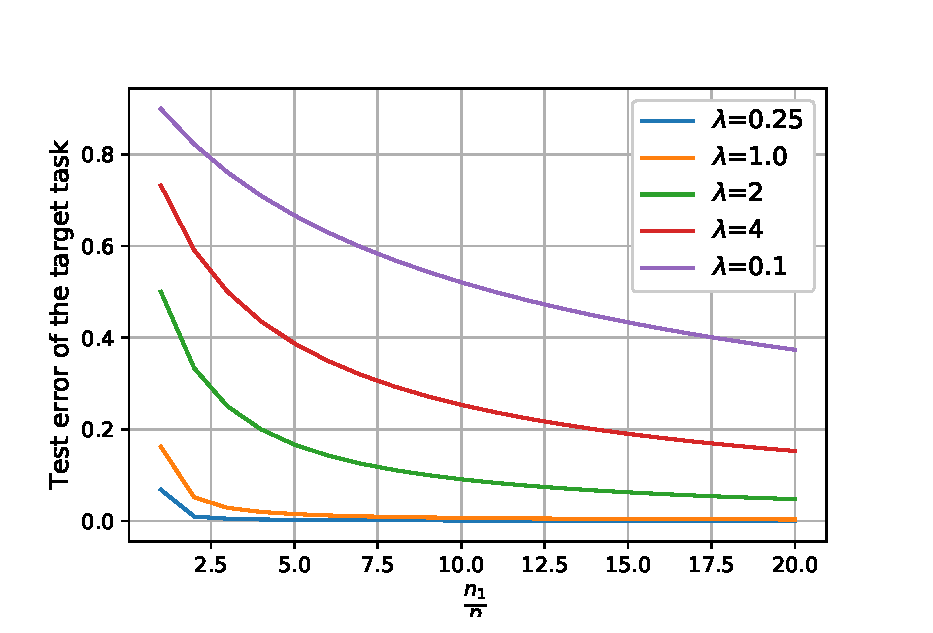
\includegraphics[width=0.9\textwidth]{figures/scaling.eps}
		\caption{When $\Sigma_1 = \Sigma_2 / \lambda$.}
		\label{fig_te_scaling}
	\end{minipage}\hfill
	\begin{minipage}{0.48\textwidth}
		\centering
		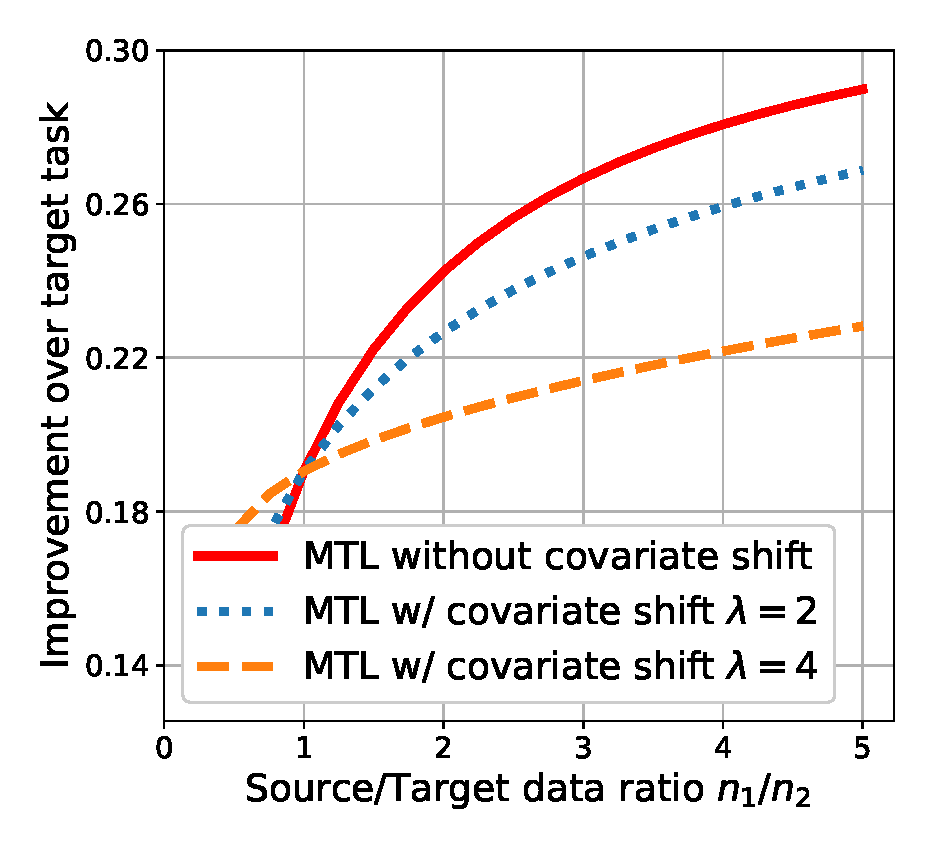
\includegraphics[width=0.9\textwidth]{figures/complementary.eps}
		\caption{When $\Sigma_1$ and $\Sigma_2$ are complementary. The number of target task data points is $n_2 = 4p$.}
		\label{fig_te_complement}
	\end{minipage}
\end{figure}


\paragraph{Extending the intuition to the general case.}
When there is model shift, i.e. $\beta_s = \beta_t$, we can still use Theorem \ref{thm_model_shift} (and Proposition \ref{prop_model_shift_tight}) to get the result.
\begin{itemize}
	\item \textbf{The effect of covariate shift:}
	\item \textbf{The effect of data ratio:}
\end{itemize}



\subsection{Gains of Transfer Learning over Multi-Task Training}



\section{The Case with Many Tasks of the Same Covariates}
















\section{The Case with Many Tasks of the Same Covariates}

In this section we consider the setting with $k$ many that have the same covariates.
Since every task has the same number of data points as well as the same covariance, the only differences between different tasks are their models $\set{\beta_i}_{i=1}^k$.
For this setting, we derive solutions for the multi-task training and the transfer learning setting that match our insights qualitatively from Section \ref{sec_denoise}.

Concretely we will consider the following problem.
\begin{align}
	f(B; W_1, \dots, W_k) = \sum_{i=1}^k \bignorm{X B W_i - Y_i}^2. \label{eq_mtl_same_cov}
\end{align}
By fixing $W_1, W_2, \dots, W_k$, we can derive a closed form solution for $B$ as
\begin{align*}
	\hat{B}(W_1, \dots, W_k) &= (X^{\top}X)^{-1} X^{\top} \bigbrace{\sum_{i=1}^k Y_i W_i^{\top}} (Z Z^{\top})^{-1} \\
	&= \sum_{i=1}^k \bigbrace{\beta_i W_i^{\top}} (ZZ^{\top})^{-1} + (X^{\top}X)^{-1}X^{\top} \bigbrace{\sum_{i=1}^k \varepsilon_i W_i^{\top}} (ZZ^{\top})^{-1}
\end{align*}
where we denote $Z\in\real^{r\times k}$ as the $k$ vectors $W_1, W_2, \dots, W_k$ stacked together.
%Now we switch $\hat{B}$ back into equation \eqref{eq_mtl_same_cov} to
Similar to Section \ref{sec_setup}, we consider minimizing the validation loss over $W_1, W_2, \dots, W_k$ provided with $\hat{B}$.

\paragraph{Jointly minimizing over all tasks.}
Denote by $\varepsilon(W) = \sum_{i=1}^k \varepsilon_i W_i^{\top}$.
We shall decompose the validation loss $\val(\hat{B}; W_1, \dots, W_k)$ into two parts.
The first part is the model shift bias, which is equal to
\begin{align*}
	\sum_{j=1}^k \bigbrace{\bignorm{\Sigma^{1/2}\bigbrace{\sum_{i=1}^k(\beta_i W_i^{\top}) (ZZ^{\top})^{-1} W_j - \beta_j}}^2}
\end{align*}
The second part is the variance, which is equal to
\begin{align*}
	& \sum_{j=1}^k \exarg{\varepsilon_i, \forall i}{\bigbrace{\bigbrace{\sum_{i=1}^k \varepsilon_i W_i^{\top}} (ZZ^{\top})^{-1} W_j}^2} \cdot {\bigtr{\Sigma(X^{\top}X)^{-1}}} \\
	=& \sigma^2 \cdot \bigtr{\Sigma (X^{\top}X)^{-1}}.
\end{align*}
Therefore we shall focus on the minimizer for the model shift bias since the variance part does not depend the weights.
Let us denote $Q\in\real^{k\times k}$ where the $(i,j)$-th entry is equal to $W_i^{\top} (ZZ^{\top})^{-1} W_j$, for any $1\le i, j\le k$.
Let $B^{\star} = [\beta_1, \beta_2, \dots, \beta_k] \in\real^{p \times k}$ denote the true model parameters.
We can now write the validation loss succinctly as follows.
\begin{align*}
	\val(\hat{B}; W_1, \dots, W_k) = \sum_{j=1}^k \bignorm{\Sigma^{1/2} \bigbrace{B^{\star} Q - \beta_j}}^2 + \sigma^2 \cdot \bigtr{\Sigma (X^{\top}X)^{-1}}
\end{align*}
From the above we can solve for $Q$ optimally as \todo{this}.

\paragraph{Minimizing over the target task alone.}
If we only minimize over the the validation loss for the target task, we shall get the following.
\begin{align*}
	\val_j(\hat{B} W_j) = \bignorm{\Sigma^{1/2}\bigbrace{\sum_{i=1}^k W_i^{\top} (ZZ^{\top})^{-1}W_j \beta_i - \beta_j}}^2
	+ \sigma^2 \cdot W_j^{\top} (ZZ^{\top})^{-1} W_j \cdot \bigtr{\Sigma (X^{\top}X)^{-1}}.
\end{align*}

From the above we can obtain three conceptual insights that are consistent with Section \ref{sec_denoise} and \ref{sec_insight}.
\begin{itemize}
	\item The de-noising effect of multi-task learning.
	\item Multi-task training vs single-task training can be either positive or negative.
	\item Transfer learning is better than the other two. And the improvement over multi-task training increases as the model distances become larger.
\end{itemize}
\section{Proof Overview of Theorem \ref{thm_model_shift}}

\paragraph{The case of two tasks.}
From \cite{WZR20}, we know that either we need to explicitly restrict the capacity $r$ of $B$ so that there is transfer between the two tasks.
Following \cite{WZR20}, for the rest of the paper, we shall consider the case when $r=1$ since there are only two tasks.
Here, equation \eqref{eq_mtl} simplifies to the following
\[ f(B; w_1, w_2) = \bignorm{X_1 B w_1 - Y_1}^2 + \bignorm{X_2 B w_2 - Y_2}^2, \]
where $B\in\real^p$ and $w_1, w_2$ are both real numbers.
To solve the above, suppose that $w_1, w_2$ are fixed, by local optimality, we solve $B$ as
\begin{align*}
	\hat{B}(w) &= (w_1^2 X_1^{\top}X_1 + w_2^2 X_2^{\top}X_2)^{-1} (w_1 X_1^{\top}Y_1 + w_2 X_2^{\top}Y_2) \\
	&= \frac{1}{w_2} (w^2 X_1^{\top}X_1 + X_2^{\top}X_2)^{-1} (w X_1^{\top}Y_1 + X_2^{\top}Y_2) \\
	&= \frac{1}{w_2}\bigbrace{\beta_t + (w^2 X_1^{\top}X_1 + X_2^{\top}X_2)^{-1}\bigbrace{X_1^{\top}X_1(w\beta_s - w^2\beta_t) + (w X_1^{\top}\varepsilon_1 + X_2^{\top}\varepsilon_2)}},
\end{align*}
where we denote $w = w_1 / w_2$.
As a remark, when $w = 1$, we recover the linear regression estimator.

\medskip
\noindent\textit{Jointly optimizing over both tasks.}
Using a validation set that is sub-sampled from the original training dataset, we get a validation loss as follows
\begin{align}
		&\val(\hat{B}; w_1, w_2) \nonumber\\
	=& n_1 \cdot \bigbrace{\bignorm{\Sigma_1^{1/2}(w^2 X_1^{\top}X_1 + X_2^{\top}X_2)^{-1}X_2^{\top}X_2(\beta_s - w\beta_t)}^2 + \sigma^2 \cdot \bigtr{(w^2 X_1^{\top}X_1 + X_2^{\top}X_2)^{-1}\Sigma_1}} \nonumber \\
	+& n_2 \cdot \bigbrace{w^2\bignorm{\Sigma_2^{1/2}(w^2 X_1^{\top}X_1 + X_2^{\top}X_2)^{-1}X_1^{\top}X_1(\beta_s - w\beta_t)}^2 + \sigma^2 \cdot \bigtr{(w^2 X_1^{\top}X_1 + X_2^{\top}X_2)^{-1}\Sigma_2}} \label{eq_val_mtl}
\end{align}
Minimizing the above loss is akin to performing multi-task training in practice.
Let $\hat{w}$ denote the minimizer of $\val(\hat{B}; w_1, w_2)$ over $w\in\real$.
We will denote $\hat{\beta}_t^{\MTL} = w_{2}\hat{B}(\hat{w})$.

\medskip
\noindent\textit{Optimizing over the target task.} The validation loss of using $w_2 \hat{B}(w)$ for the target task is
\begin{align}
	\val(w_2\hat{B}(w)) =&~ w^2 \bignorm{\Sigma_2^{1/2}(w^2 X_1^{\top}X_1 + X_2^{\top}X_2)^{-1} X_1^{\top}X_1 (\beta_s - w \beta_t)}^2 \nonumber \\
			&~ + \sigma^2 \cdot \bigtr{(w^2 X_1^{\top}X_1 + X_2^{\top}X_2)^{-1} \Sigma_2}. \label{eq_te_mtl}
\end{align}
In the above, the first is a bias term introduced by the model shift between the source and target tasks.
The second is a variance term, which decreases monotonically as we add more and more source task data.
Let $\hat{w}$ denote the minimizer of $te(w_2 \hat{B})$ over $w\in\real$.
Note that we can obtain the value of $\te(w_1\hat{B})$ through a validation set.
We will denote $\hat{\beta}_t^{\TL} = w_2 \hat{B}(\hat{w})$.

There are two reasons for studying this setting.
First, this is akin to performing transfer learning using the hard parameter sharing architecture.
Another way to obtain $\hat{\beta}_t^{\TL}$ is that once we minimize the multi-task validation loss, we further minimize the validation loss on the target dataset, which is also known as fine-tuning in practice.

Our goal is to study under model and covariate shifts, whether multi-task learning helps learn the target task better than single-task learning.
The baseline where we solve the target task with its own data is
\begin{align*}
	te(\hat{\beta}_t^{\STL}) = \sigma^2 \cdot \bigtr{(X_1^{\top}X_1 + X_2^{\top}X_2)^{-1}}, \text{ where } \hat{\beta}_t^{\STL} = (X_2^{\top}X_2)^{-1} X_2^{\top}Y_2.
\end{align*}
Clearly, whether $\hat{\beta}_t^{\MTL}$ outperforms $\hat{\beta}_t^{\STL}$ depends on the covariate matrices, the difference of the task models, and the number of per-task data points.

\todo{connect here}

\noindent\todo{A proof outline; including the following key lemma.}
To prove Theorem \ref{thm_cov_shift}, we study the spectrum of the random matrix model:
$$Q= \Sigma_1^{1/2}  Z_1^{\top} Z_1 \Sigma_1^{1/2}  + \Sigma_2^{1/2}  Z_2^{\top} Z_2 \Sigma_2^{1/2} ,$$
where $\Sigma_{1,2}$ are $p\times p$ deterministic covariance matrices, and $X_1=(x_{ij})_{1\le i \le n_1, 1\le j \le p}$ and $X_2=(x_{ij})_{n_1+1\le i \le n_1+n_2, 1\le j \le p}$ are $n_1\times p$ and $n_2 \times p$ random matrices, respectively, where the entries $x_{ij}$, $1 \leq i \leq n_1+n_2\equiv n$, $1 \leq j \leq p$, are real independent random variables satisfying
\begin{equation}\label{eq_12moment} %\label{assm1}
\mathbb{E} z_{ij} =0, \ \quad \ \mathbb{E} \vert z_{ij} \vert^2  = 1.
\end{equation}


\begin{lemma}\label{lem_cov_shift}
	In the setting of Theorem \ref{thm_model_shift}, we have with high probability $1-{\rm o}(1)$,
\begin{align}\label{lem_cov_shift_eq}
\tr ((w^2 X_1^{\top}X_1 + X_2^{\top}X_2)^{-1}\Sigma_2) = \frac{1}{n_1+n_2}\cdot \tr \left( \frac{1}{a_1 M^\top M + a_2} \right) +\bigo{ n^{-1/2+\epsilon}},
\end{align}
	for any constant $\epsilon>0$. %, where $a_{3,4}$ are found using equations in  \eqref{m35reduced}.
	Moreover, when $n_1 = 0$, we have %we have that $a_1 = 0$ and $a_2 = (n_2-p) / n_2$, hence
	\begin{align}\label{lem_cov_shift_eq2} \bigtr{(X_2^{\top}X_2)^{-1}\Sigma_2} = \frac{p}{n_2-p} + \bigo{n^{-1/2+\epsilon}}, \end{align}
which is a well-known result for inverse Whishart matrices {\color{red}add some references}.
\end{lemma}
We will give the proof of this lemma in Section \ref{sec_maintools}.

\begin{lemma}\label{lem_minv}[\todo{ref?}]
	In the setting when $n_2 = c_2 p$ we have that as $p$ goes to infinity,
	\[ \bigtr{(X_2^{\top}X_2)^{-1}\Sigma_2} = \frac{p}{n_2 - p}. \]
\end{lemma}


\paragraph{A tighter bound for a special case.} We can get a bound tighter than Theorem \ref{thm_model_shift} as follows.

	\begin{proposition}\label{prop_model_shift_tight}
		In the setting of Theorem \ref{thm_model_shift}, assume that $\Sigma_1 =\id$,
		$\beta_t$ is i.i.d. with mean $0$ and variance $\kappa^2$ and $\beta_s - \beta_t$ is i.i.d. with mean $0$ and variance $d^2$.
		We set $\Delta_{\beta} = \bigbrace{(1 - \hat{w})^2 \kappa^2 + d^2)} \bigtr{Z}$
		and we have
		\begin{align*}
			\te(\hat{\beta}_t^{\MTL}) \le \te(\hat{\beta}_t^{\STL}) \text{ when: } & \Delta_{\vari} \ge \bigbrace{1 + \sqrt{\frac{p}{n_1}}}^4 \Delta_{\beta}, \\
			\te(\hat{\beta}_t^{\MTL}) \ge \te(\hat{\beta}_t^{\STL}) \text{ when: } & \Delta_{\vari} \le \bigbrace{1 - \sqrt{\frac{p}{n_1}}}^4 \Delta_{\beta}.
		\end{align*}
	\end{proposition}




\section{Related Work}


We refer the interested readers to several excellent surveys on multi-task and transfer learning for a comprehensive survey \cite{PY09,R17,ZY17,V20}.

\textit{Multi-task learning theory.}
Some of the earliest work on multi-task learning are Baxter \cite{B00}, Ben-David and Schuller \cite{BS03}.
Mauer \cite{M06} Generalization bounds for linear separation settings of MTL
Ben-David et al. \cite{BBCK10} provides uniform convergence bounds that combines empirical and target errors in an optimal way.
The benefit of learning multi-task representations is studied for learning certain half-spaces \cite{MPR16} and sparse regression \cite{LPTV09,LPVT11}.
Our work is closely related to Wu et al. \cite{WZR20}.
While Wu et al. provide generalization bounds to show that adding more labeled helps learn the target task more accurately, their results do not apply to explain the phenomena of negative transfer.

% Adding a regularization over $B$, e.g. .
\textit{Multi-task learning methodology.}
Ando and Zhang \cite{AZ05} introduces an alternating minimization framework for learning multiple tasks.
Argyriou et al. \cite{AEP08} presents a convex algorithm which learns common sparse representations across a pool of related tasks.
Evgeniou et al. \cite{EMP05} develops a framework for multi-task learning in the context of kernel methods.
\cite{KD12} observed that controlling the capacity can outperform the implicit capacity control of adding regularization over $B$.
The multi-task learning model that we have focused on is based on the idea of hard parameter sharing \cite{C93,R17}.
We believe that the technical tools we have developed can also be applied to many other multi-task learning models.

\textit{Random matrix theory.} The random matrix theory tool and related proof of this paper fall into a paradigm of the so-called local law of random matrices \cite{erdos2017dynamical}. For a sample covariance matrix $X^\top X$ with $\Sigma=\id$, such a local law was proved in \cite{isotropic}. It was later extended to sample covariance matrices with non-identity $\Sigma$ \cite{Anisotropic}, and separable covariance matrices \cite{yang2019spiked}. On the other hand, one may derive the asymptotic result in Theorem \ref{lem_cov_shift_informal} with error $\oo(1)$ using free addition of two independent random matrices in free probability theory \cite{nica2006lectures}. To the best of my knowledge, we do not find an {\it explicit result} for the sum of two sample covariance matrices with general covariates in the literature.



\section{Conclusions and Discussions}

%\section{Extensions to the Sparse Setting}
One important case is the sparse case, where we assume that the $\beta_i$'s are sparse in the sense
that each $\beta_i$ is in a subspace of dimension $k_i\ll p$. In other words,
$$\beta_i = \sum_{j=1}^{k_i} a^{(i)}_j v^{(i)}_j,$$
where $\{v^{(i)}_j\}$ is a set of $k_i$ orthonormal vectors. For $X_i= Z_i \Sigma_i^{1/2}$, we have
$$ X_i \beta_i = Z_i \Sigma_i^{1/2}\beta_i=  Z_i \Sigma_i^{1/2}P_i\beta_i,\quad P_i:= \sum_{j=1}^{k_i}v_j^{(i)}(v_j^{(i)})^\top.$$
Then we have
$$\frac{1}{n_i}\mathbb E\left[P_i \Sigma_i^{1/2} Z_i^T Z_i \Sigma_i^{1/2}P_i\right]=P_i \Sigma_i P_i.$$
Hence our analysis will be valid with projected covariance matrices $P_i \Sigma_i P_i$. Moreover, due to the sparsity assumption, it is natural to have restricted isometry property:
$$\frac{1}{n_i} P_i \Sigma_i^{1/2} Z_i^T Z_i \Sigma_i^{1/2}P_i \approx P_i \Sigma_i P_i.$$
Finally, for our analysis it is not necessary to assume that $\beta_T$ is sparse for the target.




\bibliographystyle{plain}
\bibliography{rf}

\appendix

\section{Proofs of Theorem \todo{bla}}

The proofs of Theorem \ref{thm_model_shift} and Theorem \ref{thm_model_shift_neg} involve two parts.

\paragraph{Part I: Bounding the bias from model shift.}
We relate the first term in equation \eqref{eq_te_model_shift} to $\Delta_{\beta}$.
\begin{proposition}\label{prop_model_shift}
	In the setting of Theorem \ref{thm_model_shift}, we have that
	\begin{align*}
		\bigbrace{1 - {4\sqrt{\frac{p}{n_1}}} - {2\frac{p}{n_1}}} \Delta_{\beta}
		\le \bignorm{\Sigma_2^{1/2} (X_1^{\top}X_1 + X_2^{\top}X_2)^{-1}X_1^{\top}X_1(\beta_s - \beta_t)}^2
		\le \bigbrace{1 + \sqrt{\frac{p}{n_1}}}^4 \Delta_{\beta}.
	\end{align*}
	For the special case when $\Sigma_1 = \id$ and $\beta_s - \beta_t$ is i.i.d. with mean $0$ and variance $d^2$, we further have
	\begin{align*}
		\bigbrace{1 - \sqrt{\frac{p}{n_1}}}^4 \Delta_{\beta}
		\le \bignorm{\Sigma_2^{1/2} (X_1^{\top}X_1 + X_2^{\top}X_2)^{-1}X_1^{\top}X_1(\beta_s - \beta_t)}^2.
	\end{align*}
\end{proposition}

\begin{proof}
	The proof follows by applying equation \eqref{eq_isometric}.
	Recall that $X_1^{\top}X_1 = \Sigma_1^{1/2}Z_1^{\top}Z_1\Sigma_1^{1/2}$.
	Denote by $\cE = Z_1^{\top}Z_1 - {n_1}\id$.
	Let $K = (X_1^{\top}X_1 + X_2^{\top}X_1)^{-1}$.
	Let $\alpha = \bignorm{\Sigma_2^{1/2} K \Sigma_1 (\beta_s - \beta_t)}^2$.
	We have
	\begin{align}
		& \bignorm{\Sigma_2^{1/2}(X_1^{\top}X_1 + X_2^{\top}X_2)^{-1}X_1^{\top}X_1(\beta_s - \beta_t)}^2 \nonumber \\
		= &{n_1^2}{}\alpha + {2n_1}(\beta_s - \beta_t)^{\top}\Sigma_1^{1/2}\cE\Sigma_1^{1/2}K \Sigma_2 K \Sigma_1 (\beta_s - \beta_t)
		+ \bignorm{\Sigma_2^{1/2} K \Sigma_1^{1/2}\cE \Sigma_1^{1/2}(\beta_s - \beta_t)}^2 \label{eq_lem_model_shift_1}\\
		\le& n_1\bigbrace{{n_1^2}{} + \frac{2n_1}p(p + 2\sqrt{{n_1}p}) + (p + 2\sqrt{{n_1}p})^2} \alpha = n_1^2\bigbrace{1 + \sqrt{\frac{p}{n_1}}}^4 \alpha. \nonumber
	\end{align}
	Here we use the following on the second term in equation \eqref{eq_lem_model_shift_1}
	\begin{align*}
		& \bigabs{(\beta_s - \beta_t)^{\top} \Sigma_1^{1/2} \cE \Sigma_1^{1/2} K \Sigma_2 K \Sigma_1 (\beta_s - \beta_t)} \\
		= & \bigabs{\bigtr{\cE \Sigma_1^{1/2}K\Sigma_2 K \Sigma_1(\beta_s - \beta_t)(\beta_s - \beta_t)^{\top} \Sigma_1^{1/2}}} \\
		\le & \norm{\cE} \cdot \bignormNuclear{\Sigma_1^{1/2} K \Sigma_2 K \Sigma_1 (\beta_s - \beta_t) (\beta_s - \beta_t)^{\top} \Sigma_1^{1/2}} \\
		\le & n_1 \bigbrace{2\sqrt{\frac{p}{n_1}} + \frac{p}{n_1}} \cdot \bignormNuclear{\Sigma_1^{1/2} K \Sigma_2 K \Sigma_1 (\beta_s - \beta_t)(\beta_s - \beta_t)^{\top} \Sigma_1^{1/2}} \tag{by equation \eqref{eq_isometric}} \\
		=   & n_1 \bigbrace{2\sqrt{\frac{p}{n_1}} + \frac{p}{n_1}} \alpha \tag{since the matrix inside is rank 1}
	\end{align*}
	The third term in equation \eqref{eq_lem_model_shift_1} can be bounded similarly.

	For the other direction, we simply note that the third term in equation \eqref{eq_lem_model_shift_1} is positive.
	And the second term is bigger than $-2n_1^2(2\sqrt{\frac{p}{n_1}} + \frac{p}{n_1}) \alpha$ using equation \eqref{eq_isometric}.
\end{proof}


%	\begin{align}
%		\left(\frac{n_2}{n_1+n_2}\frac1{a_1^2}- \frac1{n_1+n_2}\sum_{i=1}^p \frac{1}{ (a_1 + \lambda_i^2a_2)^2  }\right) a_3 -  \left(\frac1{n_1+n_2}\sum_{i=1}^p \frac{  \lambda_i^2 }{ (  a_1 + \lambda_i^2a_2)^2  }\right)a_4 &=  \frac1{n_1+n_2}\sum_{i=1}^p \frac{1 }{ (  a_1 + \lambda_i^2a_2)^2  } , \label{eq_a3} \\
%		\left( \frac{n_1}{n_1+n_2}\frac1{a_2^2} -  \frac1n\sum_{i=1}^p \frac{\lambda_i^4   }{  (a_1 + \lambda_i^2a_2)^2  }\right)a_4 -\left( \frac1 {n_1+n_2}\sum_{i=1}^p \frac{\lambda_i^2  }{  (a_1 + \lambda_i^2a_2)^2  }\right)a_3 &=   \frac1 {n_1+n_2}\sum_{i=1}^p \frac{\lambda_i^2 }{  (a_1 + \lambda_i^2a_2)^2  }. \label{eq_a4}
%	\end{align}
	%We have that
	%\begin{align*}
	%	&~ {\bignorm{\Sigma_2^{1/2} (X_1^{\top}X_1 + X_2^{\top}X_2)^{-1} X_1^{\top}X_1 %(\beta_s - \beta_t)}} \\
	%	&\le ~ \left[(\beta_s - \beta_t)^{\top}\Sigma_1^{1/2}M\frac{(1 + a_3)\id + a_4 M^{\top}M}{(a_1 + a_2 M^{\top}M)} M^{\top}\Sigma_1^{1/2} (\beta_s - \beta_t)\right]^{1/2} \\
	%	&+ \left\|M\frac{(1 + a_3)\id + a_4 M^{\top}M}{(a_1 + a_2 M^{\top}M)} M^{\top}\right\|_{op}^{1/2} \|\Sigma_1^{1/2} (\beta_s - \beta_t)\|_2 \left( 2\sqrt{\frac{p} {n_1}} + \frac{p}{n_1}\right),
	%\end{align*}
	%and
	%\begin{align*}
	%	&~ {\bignorm{\Sigma_2^{1/2} (X_1^{\top}X_1 + X_2^{\top}X_2)^{-1} X_1^{\top}X_1 (\beta_s - \beta_t)}} \\
	%	&\ge ~ \left[(\beta_s - \beta_t)^{\top}\Sigma_1^{1/2}M\frac{(1 + a_3)\id + a_4 M^{\top}M}{(a_1 + a_2 M^{\top}M)} M^{\top}\Sigma_1^{1/2} (\beta_s - \beta_t)\right]^{1/2} \\
	%	&- \left\|M\frac{(1 + a_3)\id + a_4 M^{\top}M}{(a_1 + a_2 M^{\top}M)} M^{\top}\right\|_{op}^{1/2} \|\Sigma_1^{1/2} (\beta_s - \beta_t)\|_2 \left( 2\sqrt{\frac{p} {n_1}} + \frac{p}{n_1}\right).
	%\end{align*}
	%Here in the error term $p$ can be replaced with the rank of $\Sigma_1$. Without any extra information, we can only use the fact the rank of $\Sigma_1$ is at most $p$.

\paragraph{Part II: The limit of $\bignorm{\Sigma_2^{1/2} (X_1^{\top}X_1 + X_2^{\top}X_2)^{-1}\Sigma_1 (\beta_s - \beta_t)}^2$ using random matrix theory.}
We consider the same setting as in previous subsection:
$$ X_1^{\top}X_1:=\Sigma_1^{1/2}  Z_1^T Z_1 \Sigma_1^{1/2} ,\quad X_2^{\top}X_2= \Sigma_2^{1/2}  Z_2^T Z_2 \Sigma_2^{1/2},$$
where $z_{ij}$, $1 \leq i \leq n_1+n_2\equiv n$, $1 \leq j \leq p$, are real independent random variables satisfying \eqref{eq_12moment}. For now, we assume that the random variables $z_{ij}$ are i.i.d. Gaussian, but we know that universality holds for generally distributed entries. Assume that $p/n_1$ is a small number such that $Z_1^TZ_1$ is roughly an isometry, that is, under \eqref{eq_12moment},
%\todo{
%\begin{align}\left\| Z_1^T Z_1 -  \frac{n_1}{n} I \right\| \le 2\sqrt{\frac{p}{n}} + {\frac{p}{n}} .
%\end{align}}
{\color{blue}
If we assume the variances of the entries of $Z_1$ are $1$, then we have
\begin{align}
- {n_1} \left(2\sqrt{\frac{p}{n_1}} - {\frac{p}{n_1}}\right)  \le {Z_1^T Z_1 -  n_1 \id}  \le {n_1} \left(2\sqrt{\frac{p}{n_1}} + {\frac{p}{n_1}}\right) . \label{eq_isometric}
\end{align}
}

%Then we have
%$$  \left\|X_1^{\top}X_1 (\beta_s - \beta_t)  - \frac{n_1}{n}(\beta_s - \beta_t)\right\|_2 \le C \sqrt{\frac{p}{n}} \left\| (\beta_s - \beta_t)\right\|_2. $$
\todo{(revise the following proof)} It remain to study the following expression
\begin{align*}
\frac{1}{X_1^{\top}X_1 + X_2^{\top}X_2}  \Sigma_2 \frac{1}{X_1^{\top}X_1 + X_2^{\top}X_2}  = \Sigma_2^{-1/2}\left(\frac{1}{A^T Z_1^{\top}Z_1 A + Z_2^{\top}Z_2} \right)^2 \Sigma_2^{-1/2} \\
\stackrel{d}{=} \Sigma_2^{-1/2}V \left(\frac{1}{\Lambda Z_1^{\top}Z_1 \Lambda + Z_2^{\top}Z_2} \right)^2 V^T \Sigma_2^{-1/2},
\end{align*}
where
\be  \label{eigen2}
A:=\Sigma_1^{1/2}\Sigma_2^{-1/2} = U\Lambda V^T ,\quad \Lambda=\text{diag}(\lambda_1, \cdots, \lambda_p).
\ee
Using
$$\left(\frac{1}{\Lambda Z_1^{\top}Z_1 \Lambda + Z_2^{\top}Z_2} \right)^2 =\left. \frac{\dd }{\dd z}\right|_{z=0}\frac{1}{\Lambda Z_1^{\top}Z_1 \Lambda + Z_2^{\top}Z_2 - z} ,$$
we  need to study the resolvent of
$$G(z) = \left( \Lambda Z_1^{\top}Z_1 \Lambda + Z_2^{\top}Z_2 - z \right)^{-1}.$$
Its local law can be studied as in previous subsection (be careful we need to switch the roles of $Z_1$ and $Z_2$). More precisely,  we have that
$$ G(z) \approx \diag\left( \frac{1}{-z\left( 1+ m_3(z) + \lambda_i^2 m_4(z)\right)}\right)_{1\le i \le p}= \frac{1}{-z\left( 1+ m_3(z) + \Lambda^2 m_4(z)\right)} .$$
Here $m_{3,4}(z)$ satisfy the following self-consistent equations
%$$\frac{1}{G_{ii}} \approx -z \left( 1+m_3 + d_i^2m_4 \right), \quad \frac{1}{G_{\mu\mu}} = -z(1+m_1), \ \ \mu\in \cal I_1,\quad \frac{1}{G_{\nu\nu}} = -z(1+m_2), \ \ \nu\in \cal I_2,$$
%$$m_1= \frac1n\sum_{i}G_{ii}, \quad m_2= \frac1n\sum_{i}d_i^2 G_{ii}, \quad m_3 = \frac1n\sum_{\mu\in \cal I_1} G_{\mu\mu},\quad m_4 = \frac1n\sum_{\mu\in \cal I_2} G_{\mu\mu}.$$
\begin{align}\label{m34shift}
\frac{n_2}{n}\frac1{m_3} = - z +\frac1n\sum_{i=1}^p \frac1{  1+m_3 + \lambda_i^2m_4  } ,\quad \frac{n_1}{n}\frac1{m_4} = - z +\frac1n\sum_{i=1}^p \frac{\lambda_i^2 }{  1+m_3 + \lambda_i^2m_4  } .
\end{align}
Then we calculate the derivatives of $u_3:=zm_3$ and $u_4:=zm_4$ with respect to $z$:
\begin{align}\label{dotm34}
\frac{n_2}{n}\frac1{u_3^2}u'_3 =  \frac1n\sum_{i=1}^p \frac{1+u'_3 + \lambda_i^2 u'_4}{ ( z+u_3 + \lambda_i^2u_4)^2  } ,\quad \frac{n_1}{n}\frac1{u_4^2}u'_4 =   \frac1n\sum_{i=1}^p \frac{\lambda_i^2\left(1+u'_3 + \lambda_i^2 u'_4\right) }{  (z+u_3 + \lambda_i^2u_4)^2  } .
\end{align}
We can solve the above equations to get $u'_3$ and $u'_4$. Then we have
$$ G^2(z) \approx   \frac{1 +  u_3'(z) +\Lambda^2 u'_4(z)}{ \left( z+ u_3(z) + \Lambda^2  u_4(z)\right)^2}  $$
{\cob in certain sense}.

\cob $a_3\to a_2$, $a_4\to a_1$ \nc

We now simplify the expressions for $z\to 0$ case. When $z\to 0$, we shall have
$$u_3(z)= -  {a_3} + \OO(z), \quad u_4(z)= -  a_4 + \OO(z), \quad a_3,a_4 >0.$$
For $z\to0$, the equations in \eqref{m34shift} are reduced to
\begin{align}\label{m35shift}
\frac{n_2}{n}\frac{1}{\todo{a_2}} = 1 +\frac1n\sum_{i=1}^p \frac{1}{\todo{a_2} + \lambda_i^2\todo{a_1}  } ,\quad \frac{n_1}{n}\frac1{\todo{a_1}} = 1 +\frac1n\sum_{i=1}^p \frac{\lambda_i^2 }{  \todo{a_2} + \lambda_i^2 \todo{a_1} }.
\end{align}
It is easy to see that these equations are equivalent to
\begin{align} a_1 + a_2 = 1- \gamma_n, \quad a_1 +\frac1n\sum_{i=1}^p \frac{a_1}{a_1 + a_2/\lambda_i^2}=\frac{n_1}{n}  .\end{align}
The equations in \eqref{dotm34} reduce to
\be \label{dotm34red}
\begin{split}
\left(\frac{n_2}{n}\frac1{\todo{a_2}^2}- \frac1n\sum_{i=1}^p \frac{1 }{ (  \todo{a_2} + \lambda_i^2\todo{a_1})^2  }\right) a_3 -  \left(\frac1n\sum_{i=1}^p \frac{  \lambda_i^2 }{ (  \todo{a_2} + \lambda_i^2\todo{a_1})^2  }\right)a_4 =  \frac1n\sum_{i=1}^p \frac{1 }{ (  \todo{a_2} + \lambda_i^2\todo{a_1})^2  } ,\\
 %\frac{n_1}{n}\frac1{a_4^2}b_4 =   \frac1n\sum_{i=1}^p \frac{\lambda_i^2\left(1+b_3 + \lambda_i^2 b_4\right) }{  (a_3 + \lambda_i^2a_4)^2  } , \\
 \left( \frac{n_1}{n}\frac1{a_1^2} -  \frac1n\sum_{i=1}^p \frac{\lambda_i^4   }{  (a_2 + \lambda_i^2a_1)^2  }\right)a_4 -\left( \frac1n\sum_{i=1}^p \frac{\lambda_i^2  }{  (a_2 + \lambda_i^2a_1)^2  }\right)a_3 =   \frac1n\sum_{i=1}^p \frac{\lambda_i^2 }{  (a_2 + \lambda_i^2a_1)^2  } .
\end{split}
\ee
where we denote $b_3:=u_3'(0)$ and $b_4:=u_4'(0)$. Thus we have
$$\left(\frac{1}{\Lambda Z_1^{\top}Z_1 \Lambda + Z_2^{\top}Z_2} \right)^2  = G^2(0) \approx   \frac{ 1 + b_3 + \Lambda^2  b_4}{\left( a_3 + \Lambda^2  a_4\right)^2} .$$
This gives that
\begin{align*}
& \frac{1}{X_1^{\top}X_1 + X_2^{\top}X_2}  \Sigma_2 \frac{1}{X_1^{\top}X_1 + X_2^{\top}X_2} =\Sigma_2^{-1/2}V \left(\frac{1}{\Lambda Z_1^{\top}Z_1 \Lambda + Z_2^{\top}Z_2} \right)^2 V^T \Sigma_2^{-1/2}\\
& \approx  \Sigma_2^{-1/2}V \frac{ 1 + b_3 + \Lambda^2  b_4}{\left( a_3 + \Lambda^2  a_4\right)^2}V^T \Sigma_2^{-1/2}= \Sigma_2^{-1/2}  \frac{ 1 + b_3 +  b_4 A^\top A }{\left( a_3 +   a_4 A^\top A\right)^2}\Sigma_2^{-1/2} .
\end{align*}
Hence we have
\begin{align*}
& (\beta_s - \beta_t)^{\top}X_1^{\top}X_1 \frac{1}{X_1^{\top}X_1 + X_2^{\top}X_2}  \Sigma_2 \frac{1}{X_1^{\top}X_1 + X_2^{\top}X_2} X_1^{\top}X_1 (\beta_s - \beta_t) \\
 & \approx (\beta_s - \beta_t)^{\top}\Sigma_1 \Sigma_2^{-1/2}  \frac{ 1 + a_3 +  a_4 A^\top A }{\left( a_2 +   a_1 A^\top A\right)^2}\Sigma_2^{-1/2} \Sigma_1(\beta_s - \beta_t).
\end{align*}



%Then it is equivalent to study
%$$Q:=  ( X_1^T X_1 )^{-1}   D X_2^T X_2 D ,$$
%which has the same nonzero eigenvalues of
%$$\mathcal Q:=  X_2 D ( X_1^T X_1 )^{-1} D X_2^T,$$
%i.e. $\mathcal Q$ has the same nonzero eigenvalues of $Q$, but has $(n_2-p)$ more zero eigenvalues.

%----------The following is the results on the eigenvalues, not the singular values-------------
%We are interested in the eigenvalues of
%$$(X_1^{\top}X_1)^{-1} (X_2^{\top}X_2),$$
%which is called a generalized Fisher matrix. As in the previous setting, we write out their covariance explicitly and consider
%$$  (\Sigma_1^{1/2}  Z_1^T Z_1 \Sigma_1^{1/2})^{-1}   \Sigma_2^{1/2}  Z_2^T Z_2 \Sigma_2^{1/2} ,$$
%where $\Sigma_{1,2}$ are $p\times p$ deterministic covariance matrices, and $X_1=(x_{ij})_{1\le i \le n_1, 1\le j \le p}$ and $X_2=(x_{ij})_{n_1+1\le i \le n_1+n_2, 1\le j \le p}$ are $n_1\times p$ and $n_2 \times p$ random matrices, respectively, where the entries $x_{ij}$, $1 \leq i \leq n_1+n_2\equiv n$, $1 \leq j \leq p$, are real independent random variables satisfying \eqref{eq_12moment}.
%We can study it using the linearization matrix ({\color{red}for my own purpose right now})
%$$ H = \begin{pmatrix} - z I & X_2D & 0 \\ DX_2^T & 0 & X_1^T \\ 0 & X_1 & I \end{pmatrix}, \quad G(z):=H(z)^{-1}.$$
%Then the $(1,1)$-th block is equal to $\cal G(z):=(\mathcal Q-z)^{-1}$. We denote
%\begin{equation}\label{m1m}m_1(z):=\frac1n\tr \cal G(z), \quad m(z)= \frac1p \left[ nm_1(z) + \frac{n_2-p}{z}\right].\ee
%We can show that it satisfies the following self-consistent equations together with another $m_3(z)$:
%\begin{align}\label{m13}
%\frac{n_2}{n}\frac1{m_1} = - z +\frac1n\sum_{i=1}^p \frac{d_i^2}{ m_3 + d_i^2m_1  } ,\quad \frac{n_1}{n}\frac1{m_3} = 1 +\frac1n\sum_{i=1}^p \frac{1}{   m_3 + d_i^2m_1  } .
%\end{align}
%For these two equations, we can obtain one single equation for $m_1(z)$:
%\begin{align}\label{m1}
%m_3= 1-\frac pn + zm_1, \quad \frac{n_2}{n}\frac1{m_1} = - z +\frac1n\sum_{i=1}^p \frac{d_i^2}{ 1-\frac pn + (z + d_i^2)m_1  }  .
%\end{align}
%One can solve the above equation for $m_1$ with positive imaginary parts, and then calculate $m(z)$ using \eqref{m1m}.
%
%With $m(z)$, we can define
%$$\rho_c(z):=\frac1\pi \lim_{\eta\downarrow 0} m(z).$$
%It will be a compact supported probability density which gives the eigenvalue distribution of $Q$. Moreover, we have
%$$\frac{1}{p}\tr \frac1{(\Sigma_1^{1/2}  X_1^T X_1 \Sigma_1^{1/2})^{-1}   \Sigma_2^{1/2}  X_2^T X_2 \Sigma_2^{1/2} +1}\left(\frac1{(\Sigma_1^{1/2}  X_1^T X_1 \Sigma_1^{1/2})^{-1}   \Sigma_2^{1/2}  X_2^T X_2 \Sigma_2^{1/2} +1}\right)^T \approx \int \frac{\rho_c(x)}{(x+1)^2}{\rm d}x.$$
%We know that
%$$ m(z)=\int \frac{\rho_c(x)}{ x-z}{\rm d}x.$$
%Hence we have
%$$ m'(-1)=\int \frac{\rho_c(x)}{(x+1)^2}{\rm d}x.$$
%
%Moreover, the right edge $\lambda_+$ of $\rho_c$ gives the location of the largest eigenvalue, while the left edge $\lambda_-$  of $\rho_c$ gives the location of the smallest eigenvalue. They will provide the upper and lower bounds on the operator norm:
%$$\frac{1}{1+\lambda_+}\le \frac1{(\Sigma_1^{1/2}  X_1^T X_1 \Sigma_1^{1/2})^{-1}   \Sigma_2^{1/2}  X_2^T X_2 \Sigma_2^{1/2} +1}\le \frac1{1+\lambda_-}.$$
%The edges of the spectrum can be determined by solving the following equations of $(x,m_1)$:
%$$\frac{n_2}{n}\frac1{m_1} = - x +\frac1n\sum_{i=1}^p \frac{d_i^2}{ 1-\frac pn + (x + d_i^2)m_1  } ,\quad  \frac{n_2}{n}\frac1{m_1^2} = \frac1n\sum_{i=1}^p \frac{d_i^2 (x+d_i^2)}{\left[ 1-\frac pn + (x + d_i^2)m_1 \right]^2 } .$$
%The solutions for $x$ give the locations for the edges of the spectrum.
%--------------------------------------



\paragraph{Proof of Lemma \ref{lem_cov_shift}.}

\begin{proof}
{\color{blue}(revise the following proof)} We assume that $ \Sigma_1^{-1/2}\Sigma_2$ has eigendecomposition
\be  \label{eigen}
\Sigma_1^{-1/2}\Sigma_2^{1/2} = ODO^T ,\quad D=\text{diag}(d_1, \cdots, d_p).
\ee
Then by the rotational invariance of Gaussian matrices, we have
$$\wt Q \overset{d}{=}\Sigma_1^{1/2} O \wt Q O^T \Sigma_1^{1/2},\quad \wt Q:=   X_1^T X_1  + D X_2^T X_2 D .$$
Thus we study the spectrum of $\wt Q$ instead. We define $\cal G(z):= (\wt Q-z)^{-1}$ for $z\in \C_+$. With some random matrix tools, we have that
$$\cal G(z) \approx \diag\left( \frac{1}{-z\left( 1+ m_3(z) + d_i^2 m_4(z)\right)}\right)_{1\le i \le p}= \frac{1}{-z\left( 1+ m_3(z) + D^2 m_4(z)\right)} $$
{\cob in certain sense}. Here $m_{3,4}(z)$ satisfy the following self-consistent equations
%$$\frac{1}{G_{ii}} \approx -z \left( 1+m_3 + d_i^2m_4 \right), \quad \frac{1}{G_{\mu\mu}} = -z(1+m_1), \ \ \mu\in \cal I_1,\quad \frac{1}{G_{\nu\nu}} = -z(1+m_2), \ \ \nu\in \cal I_2,$$
%$$m_1= \frac1n\sum_{i}G_{ii}, \quad m_2= \frac1n\sum_{i}d_i^2 G_{ii}, \quad m_3 = \frac1n\sum_{\mu\in \cal I_1} G_{\mu\mu},\quad m_4 = \frac1n\sum_{\mu\in \cal I_2} G_{\mu\mu}.$$
\begin{align}\label{m34}
\frac{n_1}{n}\frac1{m_3} = - z +\frac1n\sum_{i=1}^p \frac1{  1+m_3 + d_i^2m_4  } ,\quad \frac{n_2}{n}\frac1{m_4} = - z +\frac1n\sum_{i=1}^p \frac{d_i^2 }{  1+m_3 + d_i^2m_4  }
\end{align}
When $z\to 0$, we shall have
$$m_3(z)= - \frac{a_3}{z} + \OO(1), \quad m_4(z)= - \frac{a_4}{z} + \OO(1),\quad a_3,a_4>0.$$
Then for $z\to0$, the equations in \eqref{m34} are reduced to
\begin{align}\label{m35}
\frac{n_1}{n}\frac{1}{a_3} = 1 +\frac1n\sum_{i=1}^p \frac{1}{a_3 + d_i^2a_4  } ,\quad \frac{n_2}{n}\frac1{a_4} = 1 +\frac1n\sum_{i=1}^p \frac{d_i^2 }{  a_3 + d_i^2 a_4 }.
\end{align}
First, it is easy to see that these equations are equivalent to
\begin{align} a_3 + a_4 = 1- \gamma_n, \quad a_3 +\frac1n\sum_{i=1}^p \frac{a_3}{a_3 + d_i^2[(1-\gamma_n)-a_3]  }=c_n  .\end{align}
Furthermore, we have
\begin{align*}
\tr (Q^{-1}) &= \lim_{z\to 0}\tr \left[\Sigma_1^{-1/2} O \cal G(z)O^T \Sigma_1^{-1/2}\right]
=\tr \left[\Sigma_1^{-1/2} O  \left( \frac{1}{a_3 + D^2 a_4 }\right) O^T \Sigma_1^{-1/2}\right] \\
&=\tr \left[\Sigma_1^{-1/2}  \frac{1}{a_3+ \Sigma_1^{-1}\Sigma_2 a_4} \Sigma_1^{-1/2}\right]=\tr \left[ \frac{1}{a_3\Sigma_1 + a_4\Sigma_2 } \right].
\end{align*}
\end{proof}

%\section{The Case of Two Tasks}\label{sec_defspike}
%We denote task 1 as the source, i.e. $\beta_1 = \beta_s$.
%\subsection{Covariate Shift}
%\subsection{Model Shift}


\input{appd}

%\appendix




\end{document}
